% !TEX encoding = UTF-8 Unicode

% This is a simple template for a LaTeX document using the "article" class.
% See "book", "report", "letter" for other types of document.

%%%%%%%%%%%%%%%%%%%%%%%%%%%%%%%%%%%%%
%
% Template para producir documentos "camera ready" para Anales de la AFA
% 
%  No se debería tener que modificar nada del siguiente preámbulo, donde están 
%  las customizaciones para adaptar la clase "article" a los Anales AFA.
%
%%%%%%%%%%%%%%%%%%%%%%%%%%%%%%%%%%%%%
\documentclass[10pt,twocolumn]{article} 

\usepackage[utf8]{inputenc} % set input encoding (not needed with XeLaTeX)
\usepackage[spanish]{babel}


%%% DIMENSIONES DE LA PÁGINA
\usepackage{geometry} 
\geometry{a4paper} 
 \geometry{top=2.25cm} 
 \geometry{bottom=2.25cm} 
 \geometry{left=2.5cm} 
 \geometry{right=2cm} 


%%% PACKAGES
\usepackage{graphicx} 
\usepackage{paralist} % very flexible & customisable lists (eg. enumerate/itemize, etc.)
\usepackage{verbatim} % adds environment for commenting out blocks of text & for better verbatim
\usepackage{subfig} % make it possible to include more than one captioned figure/table in a single float
\usepackage{lipsum} 
\usepackage{multirow} 
\usepackage{hyperref}
\usepackage[superscript]{cite}  %REFERENCIAS EN SUPERÍNDICE

% Ajusta los captions de tablas y figuras a italics
\usepackage[format=plain,
            labelfont=it,
            textfont=it]{caption}
% These packages are all incorporated in the memoir class to one degree or another...

%%% HEADERS & FOOTERS
\usepackage{fancyhdr} % This should be set AFTER setting up the page geometry
\usepackage{xurl}
\pagestyle{fancy} % options: empty , plain , fancy
\renewcommand{\headrulewidth}{0pt} % customise the layout...
\lhead{}\chead{}\rhead{}
\lfoot{}\cfoot{\thepage}\rfoot{}
%\renewcommand{\thefootnote}{\fnsymbol{footnote}}

\usepackage{varwidth}
\usepackage{authblk}
\newcommand{\filiacion}[2]{\affil[#1]{\protect\begin{varwidth}[t]{\linewidth}\protect\centering \normalfont#2 \protect\end{varwidth}}}
\newcommand{\autor}[2]{\author[#1]{\bf #2}}
\newcommand{\corresponding}[2]{\author[#1]{\bf #2\thanks{}}}
\newcommand\cauthemail[1]{\footnotetext{#1}}
\newcommand{\fecha}[1]{\date{\vspace{-1ex}\small{#1}}}
\newcommand{\titulo}[2]{\title{\bf{\large{#1 \\ \vspace{1.5ex} #2 }}}}
\newcommand{\esresumen}[1]{\small{#1 \par}\vspace{1.5ex}}
\newcommand{\pclaves}[1]{\small{\emph{#1} \par}\vspace{1.5ex}}
\newcommand{\enresumen}[1]{\small{#1 \par}\vspace{1.5ex}}
\newcommand{\keywords}[1]{\small{\emph{#1} \par}\vspace{1.5ex}}



%%% APARIENCIA DE TITULOS, SECCIONES Y SUBSECCIONES
\usepackage{sectsty}
\allsectionsfont{\fontsize{10}{12}\sffamily\bfseries\upshape} % (See the fntguide.pdf for font help)

\usepackage{titlesec}
\titlespacing*{\section}{0pt}{1.5ex}{0.8ex}
\titlespacing*{\subsection}{0pt}{1.2ex}{0.6ex}
\setcounter{secnumdepth}{1}   %no numera las subsecciones

\usepackage[nottoc,notlof,notlot]{tocbibind} % Put the bibliography in the ToC
\usepackage[titles,subfigure]{tocloft} % Alter the style of the Table of Contents
\renewcommand{\cftsecfont}{\rmfamily\mdseries\upshape}
\renewcommand{\cftsecpagefont}{\rmfamily\mdseries\upshape} % No bold!
\renewcommand\thesection{\Roman{section}}
\renewcommand\thesubsection{}



%%% PARA EL FORMATO DE TABLAS
\usepackage{booktabs} % for much better looking tables
\usepackage{array} % for better arrays (eg matrices) in maths
\makeatletter
\newcommand{\thickhline}{%
    \noalign {\ifnum 0=`}\fi \hrule height 1.5pt
    \futurelet \reserved@a \@xhline
}
\newcolumntype{"}{@{\hskip\tabcolsep\vrule width 1pt\hskip\tabcolsep}}
\makeatother
\newcolumntype{L}[1]{>{\raggedright\let\newline\\\arraybackslash\hspace{0pt}}m{#1}}
\newcolumntype{C}[1]{>{\centering\let\newline\\\arraybackslash\hspace{0pt}}m{#1}}
\newcolumntype{R}[1]{>{\raggedleft\let\newline\\\arraybackslash\hspace{0pt}}m{#1}}

\renewcommand\spanishtablename{Tabla}  

% Corresponding author
\usepackage[table,xcdraw,dvipsnames]{xcolor}
\makeatletter
\renewcommand\@biblabel[1]{#1.}
\makeatother

\pagestyle{empty}

%%%%%% En principio no debería hacer falta modificar nada por encima de esta línea

%%%%%%%%%%%%%%%%%%%%%%%%%%%%%%%%%%%%%%%

%%% El contenido del documento comienza a partir de acá 

%título del trabajo: en el primer campo en castellano, en el segundo en inglés
\titulo{ANÁLISIS DE LA IRRADIANCIA SOLAR UV PARA LA SÍNTESIS DE PRE-VITAMINA D\textsubscript{3} EN LA PIEL, EN ROSARIO, ARGENTINA}{ANALYSIS OF THE UV SOLAR IRRADIANCE FOR THE SYNTHESIS OF PRE-VITAMIN D\textsubscript{3} ON THE SKIN, IN ROSARIO, ARGENTINA}

\corresponding{1}{Adriana Ipiña}
\autor{2}{Gamaliel López-Padilla}
\autor{3}{Ana Laura Fisanotti}
\autor{4}{Montserrat Dávalos}
\autor{1}{Rubén D. Piacentini}

%afiliaciones: se pueden combinar
\filiacion{1}{Instituto de Física Rosario – Universidad Nacional Rosario – Consejo Nacional de Investigaciones Científicas y Técnicas, 27 de Febrero 210BIS – (S2000EKF) Rosario – Argentina.}
\filiacion{2}{Facultad de Ciencias Físico Matemáticas – Universidad Autónoma de Nuevo León, Pedro de Alba S/N - Ciudad Universitaria San Nicolás de los Garza (66451) – México.}
\filiacion{3}{Facultad de Ciencias Médicas - Universidad Nacional Rosario - Santa Fe 3100 (S2002KKT) Rosario - Argentina}
\filiacion{4}{Investigadora Independiente, Monterrey (64810) - México}

\fecha{Recibido: xx/xx/xx; Aceptado: xx/xx/xx} %No modificar


\setcounter{Maxaffil}{0}
\renewcommand\Affilfont{\itshape\small}


\begin{document}

\renewcommand{\abstractname}{}
\twocolumn[
  \begin{@twocolumnfalse}
    \maketitle
    \begin{abstract}\vspace{-12ex}
      \centering\begin{minipage}{\dimexpr\paperwidth-6cm}

        %Abstract en castellano
        \esresumen{En los últimos años, el estudio de la vitamina D ha aumentado debido al incremento en la incidencia de personas que presentan niveles deficientes de esta vitamina. Pocos alimentos contienen vitamina D\textsubscript{3} de manera natural, siendo la principal fuente de obtención la radiación solar ultravioleta (UV), la cual desencadena el mecanismo de la síntesis de la vitamina D en la parte superficial de la piel. En este estudio se determinó la irradiancia solar UV efectiva para la síntesis de pre-vitamina D\textsubscript{3} en la ciudad de Rosario, Argentina, utilizando tres métodos: a) Coeficiente de proporcionalidad, b) Ecuación de Herman y c) Modelo TUV. Los valores se compararon para condiciones de cielo despejado al mediodía solar. Se calcularon los Tiempos de Exposición Solar (TES) para obtener las dosis mínimas de radiación solar UV para sintetizar pre-vitamina D\textsubscript{3} y suficiente para producir eritema, en el periodo junio 2019 - mayo 2020. Se discute la variación de los TES para alcanzar una dosis mínima para la síntesis de pre-vitamina D\textsubscript{3} y aparición de eritema con una fotoexposición del 25\% de la superficie corporal (la cara, el cuello y los brazos). }
        \pclaves{Palabras Clave: radiación solar UV, vitamina D, eritema, tiempos de exposición solar, Argentina.} %palabras clave

        %Abstract en inglés
        \enresumen{In the last years, the study of vitamin D has raised due to the increase in the incidence of people with deficient levels of this vitamin. Few foods contain it naturally, being the main source of obtaining the ultraviolet solar radiation, which triggers the mechanism of the synthesis of vitamin D on the surface skin. In this study, the effective UV solar irradiance for the synthesis of pre-vitamin D\textsubscript{3} was determined in Rosario city, Argentina, using three methods: a) Coefficient of proportionality, b) Herman equation and c) TUV model. The values were compared in clear sky conditions at solar noon. The Solar Exposure Times (TES) were calculated to obtain the minimum doses for the synthesis of pre-vitamin D\textsubscript{3} and enough to produce erythema, in the period june 2019 - may 2020. It is discussed the variation of the TES reaching the minimum dose of pre-vitamin D\textsubscript{3} and erythema with a photoexposure of 25\% of the body (face, neck and arms).}
        \keywords{Keywords: UV solar radiation, vitamin D, erythema, solar exposure times, Argentina.}  %key words

      \end{minipage}
      \vspace{4ex}
    \end{abstract}
  \end{@twocolumnfalse}
]
\thispagestyle{empty}

\setcounter{footnote}{1}
\cauthemail{ipina@ifir-conicet.gov.ar}  % Dirección de correo electrónico del corresponding author
\section{INTRODUCCIÓN}
La vitamina D es una hormona que interviene en múltiples procesos en el cuerpo humano. Los más conocidos (denominados \emph{clásicos}), tienen lugar en el metabolismo fosfocálcico, regulando los niveles en sangre de calcio y fosfato mediante distintos mecanismos. A medida que se fue avanzando con las investigaciones, se atribuyeron muchas más funciones a la vitamina D (denominadas \emph{no clásicas}), tales como la inmunomodulación y el control de la presión arterial, entre otras \cite{bikle_2014,zuluga_2011,pozzo_2005}. Además, su deficiencia se asoció a diferentes enfermedades, como la sarcopenia, el Parkinson, el Alzheimer y la artritis reumatoidea \cite{pozzo_2005,Afzal_2013,Kravietz_2017,Ishikawa_2016}. Incluso se la ha asociado a formas más graves de la enfermedad por COVID-19 \cite{Mercola2020}.

La principal fuente de vitamina D es la síntesis en la piel producida por la radiación solar UV, ya que muy pocos alimentos la contienen de manera natural\cite{Biesalski_2002}. La radiación solar UV que llega a la superficie terrestre varía en función de la composición atmosférica (especialmente O\textsubscript{3} estratosférico y troposférico), la ubicación geográfica, la hora del día y los días del año. El rango UV es el más energético por fotón incidente (280-400 nm). Este rango espectral desencadena las reacciones fotoquímicas fundamentales en los precursores de la vitamina D. En el caso de los vegetales, se sintetiza vitamina D\textsubscript{2} (ergocalciferol) a partir del ergosterol, mientras que en los seres humanos se forma vitamina D\textsubscript{3} a partir del 7-dehidrocolesterol (7-DHC) que se encuentra en las membranas plasmáticas de los queratinocitos de la epidermis y en los fibroblastos de la dermis.\cite{2002,brunser_radiacion_2005,Olds2008} Cuando este último interactúa con los rayos UV sufre cambios conformacionales, dando como resultado la pre-vitamina D, la cual rápidamente se transforma a vitamina D\textsubscript{3} (colecalciferol) y se une a una proteína transportadora de la sangre. Sin embargo, para ejercer sus efectos la vitamina D debe sufrir dos hidroxilaciones. La primera se da en el riñón, formando la 25-hidroxi-vitamina D (calcidiol), y la segunda tiene lugar en el hígado, donde finalmente obtenemos la 1-25-dihidroxi-vitamina D (calcitriol) o, en otras palabras, la vitamina D activa.\cite{Holick_1989}


Por otro lado, la sobreexposición solar UV también puede producir efectos nocivos a largo plazo, que van desde el fotoenvejecimiento, fotodermatosis hasta cánceres de piel y cataratas.\cite{Gilaberte2011,Modenese2016} Por esta razón es importante conocer los Tiempos de Exposición Solar (TES) para iniciar la síntesis de la vitamina D, sin provocar un daño a la piel (\emph{e.g.} eritema). Para calcular los TES que producen un efecto biológico específico, se utiliza la definición de la dosis efectiva:
\begin{equation}
  Dosis=\int_{t_1}^{t_2} \int_{250nm}^{400nm} E_\lambda\cdot S_\lambda d\lambda dt = \int_{t_1}^{t_2}E_tdt \label{eq:dosis}
\end{equation}
donde E$_\lambda$ es la irradiancia solar espectral a nivel del suelo y S$_\lambda$ es el espectro de acción, que puede ser para: la síntesis de la pre-vitamina D\textsubscript{3} o generación de eritema. La irradiancia efectiva E\textsubscript{t}, representa la irradiancia de pre-vitamina D\textsubscript{3} (E\textsubscript{vitD}) o la irradiancia eritémica (E\textsubscript{er}) según sea el caso. La integral de estas irradiancias de un tiempo t\textsubscript{1} a t\textsubscript{2}, define las Dosis en unidades de J/m\textsuperscript{2}.
La Dosis Eritemica Mínima (MED por sus siglás en inglés) tiene un valor en la clasificación de Fitzpatrick de 250 J/m\textsuperscript{2} para un fototipo de piel II.\cite{Fitzpatrick1988} De manera análoga, la Dosis Mínima para generar los niveles adecuados de vitamina D\textsubscript{3} (MDD por sus siglas en inglés) es de 34 J/m\textsuperscript{2} con una exposición de cuerpo completo y de 136 J/m\textsuperscript{2} con una exposición del 25\% del cuerpo (brazos, cuello y cara).\cite{UVDoses, Fioletov_2010} La MDD también se puede aproximar en términos de $\frac{1}{4}$MED (63 J/m\textsuperscript{2}) para un fototipo II\cite{Dowdy_2010}. En este trabajo se presenta la estimación de la E\textsubscript{vitD}, mediante tres métodos: Coeficiente de proporcionalidad,\cite{UVDoses} Ecuación de Herman\cite{Herman2010} y Modelo TUV.\cite{Madronich1987} En particular, se utiliza el modelo TUV en la determinación de los TES (t\textsubscript{2}-t\textsubscript{1}) para acumular 1MED, $\frac{1}{4}$MED y 1MDD en la ciudad de Rosario, Argentina.

\section{MATERIALES Y MÉTODOS}
Los datos de la columna total de ozono (O\textsubscript{3}) provienen de la Colección 3, OMTD3 v8.5, en Unidades Dobson (DU), medidos por el Instrumento de Monitoreo de Ozono (OMI) para las coordenadas de la ciudad de Rosario, Argentina. A bordo del satélite AURA-NASA, OMI realiza observaciones diarias en una superficie de 13x24 Km\textsuperscript{2} en el nadir, disponible en \href{(disc.gsfc.nasa.gov)}{\url{disc.gsfc.nasa.gov}}. Para las mediciones \emph{in situ} de E$_\lambda$ se utilizó un espectroradiómetro Optronic-OL756 con esfera integradora y para el índice UV, la estación meteorológica Davis. Ambos instrumento se encuentran ubicados en el Instituto de Física Rosario (CONICET-UNR), en la ciudad de Rosario.

\begin{figure}[ht]
  \centering
  \includegraphics[scale=0.4]{factores.jpg}
  \caption{a)Espectros de acción de pre-vitamina D\textsubscript{3} y eritémica, e irradiancia espectral solar medida en cielo despejado, cerca de los solsticios de verano (28/Dic/2011) e invierno (23/Jun/2011), en la ciudad de Rosario. b) Irradiancia ponderada por cada espectro de acción y estación del año.}
  \label{fig:factores}
\end{figure}

\section{Coeficiente de proporcionalidad}
La Commission Internationale de l’Eclairage (CIE) y la World Meteorological Organization (WMO) reportaron la siguiente relación:

\begin{equation}
  E_{vitD} = k \cdot E_{er}
  \label{ee:CIE}
\end{equation}
\begin{table*}[ht]
  \centering
  \caption{Coeficientes\cite{Herman2010} para obtener U$(\theta)$;RAF $(\theta)= \frac{a+c\theta^2+e\theta^4}{1+b\theta^2+d\theta^4+f\theta^6}$}
  \label{table::parametros}
  \begin{tabular}{lll}
    \hline
      & \multicolumn{1}{c}{U}      & \multicolumn{1}{c}{RAF}     \\ \hline
    a & 0.9659616883022778         & 1.349378286522954           \\
    b & 0.0001089314449687077      & -0.0002926808443875372      \\
    c & -0.0002681987275053843     & -0.0003059282407232034      \\
    d & 1.410783665933483E$^{-8 }$ & 2.879164470755759E$^{-8}$   \\
    e & 1.894213900598701E$^{-8 }$ & 1.920553492457117E$^{-8}$   \\
    f & 1.695104643516458E$^{-12}$ & -8.580442654658103E$^{-13}$ \\ \hline
  \end{tabular}
\end{table*}

donde \emph{k} tiene dos valores distintos en verano e invierno para una ciudad del hemisferio sur.\cite{UVDoses} En este trabajo, los valores de \emph{k} fueron obtenidos calculando E\textsubscript{er} y E\textsubscript{vitD} por medio de la Ec. \ref{eq:dosis} y las mediciones de E$_\lambda$ realizadas bajo cielo despejado en verano e invierno (Figura \ref{fig:factores}). Posteriormente, la sustitución de E\textsubscript{er} y E\textsubscript{vitD} en la Ec. \ref{ee:CIE} determina $k$=1.6 en invierno y de $k=2$ en verano. Finalmente los valores diarios de E\textsubscript{vitD} para ambas épocas del año (21/Jun/2019 - 20/Sep/2019 invierno y 21/Dic/2019 - 20/Mar/2020 verano) se estimaron a partir de la E\textsubscript{er}. Esta irradiancia eritémica se deriva del índice UV medido al mediodía solar en cielo despejado por la estación Davis. El índice UV es internacionalmente reconocido como medida de riesgo, en una escala de 0 a 20 (o más) y resulta de multiplicar E\textsubscript{er} por 40 m$^2$/W.

\section{Ecuación de Herman}
Herman\cite{Herman2010} estableció una ecuación general de E\textsubscript{vitD} para cualquier lugar geográfico:
\begin{equation}
  E_{vitD}=U\left(\frac{O_3}{200}\right)^{-RAF}
  \label{eq:evitd}
\end{equation}
donde el O\textsubscript{3} es la columna total de ozono, RAF es el Factor de Amplificación de Radiación y U es una función de ajuste, estos dos últimos dependientes el ángulo cenital solar $(\theta)$. La E\textsubscript{vitD} en esta ecuación depende de la columna total de O\textsubscript{3} en el sitio en cuestión y de las funciones RAF y U, que a su vez dependen del ángulo cenital (relacionado a la hora del día). Los coeficientes de U y RAF se muestran en la Tabla \ref{table::parametros}, los cuales fueron obtenidos ejecutando el modelo TUV.

\section{Modelo TUV}
El modelo Tropospheric Ultraviolet Radiation (TUV)\cite{Madronich1987} emplea la ecuación de transferencia radiativa para obtener la E$_\lambda$ a nivel del suelo, en los rangos ultravioleta, visible e infrarrojo cercano. El modelo incorpora el perfil de aerosoles cuya profundidad óptica (AOD) es de 0.34 a 340 nm (desde 5.24 km al espacio) y un perfil de O\textsubscript{3} correspondiente a la atmósfera estándar de EE. UU. Entre los datos de entrada más relevantes se encuentran las coordenadas del lugar (latitud, longitud y altura sobre el nivel del mar), AOD a 550 nm, reflectividad del suelo, albedo de dispersión simple, coeficiente de Angstrom, fecha y hora del día. La columna total de O\textsubscript{3} toma la medición diaria del instrumento OMI. Cabe destacar que esta medición satelital podría estar subestimada en ciudades muy contaminadas (\emph{e.g.} Santiago de Chile) y tener diferencias significativas con respecto a las mediciones terrestres.

Con el modelo TUV también se calcularon los valores de E\textsubscript{vitD} y E\textsubscript{er} para las coordenadas de la ciudad de Rosario (32.95°S, 60.62°W, 25 m snm). Las estimaciones se realizaron diariamente al mediodía solar local (entre las 12:00 - 13:00 h) en el periodo junio 2019 - mayo 2020.

\section{Cálculo de los TES}
Los valores de E\textsubscript{vitD} y E\textsubscript{er} derivados del modelo TUV fueron utilizados como base para calcular los TES. La Ec. \ref{eq:dosis} fue resuelta sistemáticamente por un código en \emph{Python} comenzando a la hora de máxima intensidad solar ($t_1$) y terminando ($t_2$) al alcanzar: 1MED, $\frac{1}{4}$MED y 1MDD. Este proceso se repitió día a día, determinando el intervalo de tiempo ($t_2-t_1$) para generar las dosis a lo largo de todo el periodo.

\section{RESULTADOS}
La irradiancia pre-vitamina D\textsubscript{3} calculada al mediodía solar empleando los tres métodos se muestra en la Fig. \ref{fig:previtamin}. Como puede observarse, existe una alta similitud entre los resultados obtenidos con la Ec. de Herman y el modelo TUV. La diferencia relativa promedio fue de 3.6\% en verano y de 0.4\% en invierno, respecto al TUV. Mientras que las diferencias relativas en razón del Coeficiente de proporcionalidad con el TUV y la Ec. de Herman fueron de: 8.5\% y 8.4\% en invierno, así como de 20.8\% y 17.1\% en verano, respectivamente.

\begin{figure}[ht]
  \centering
  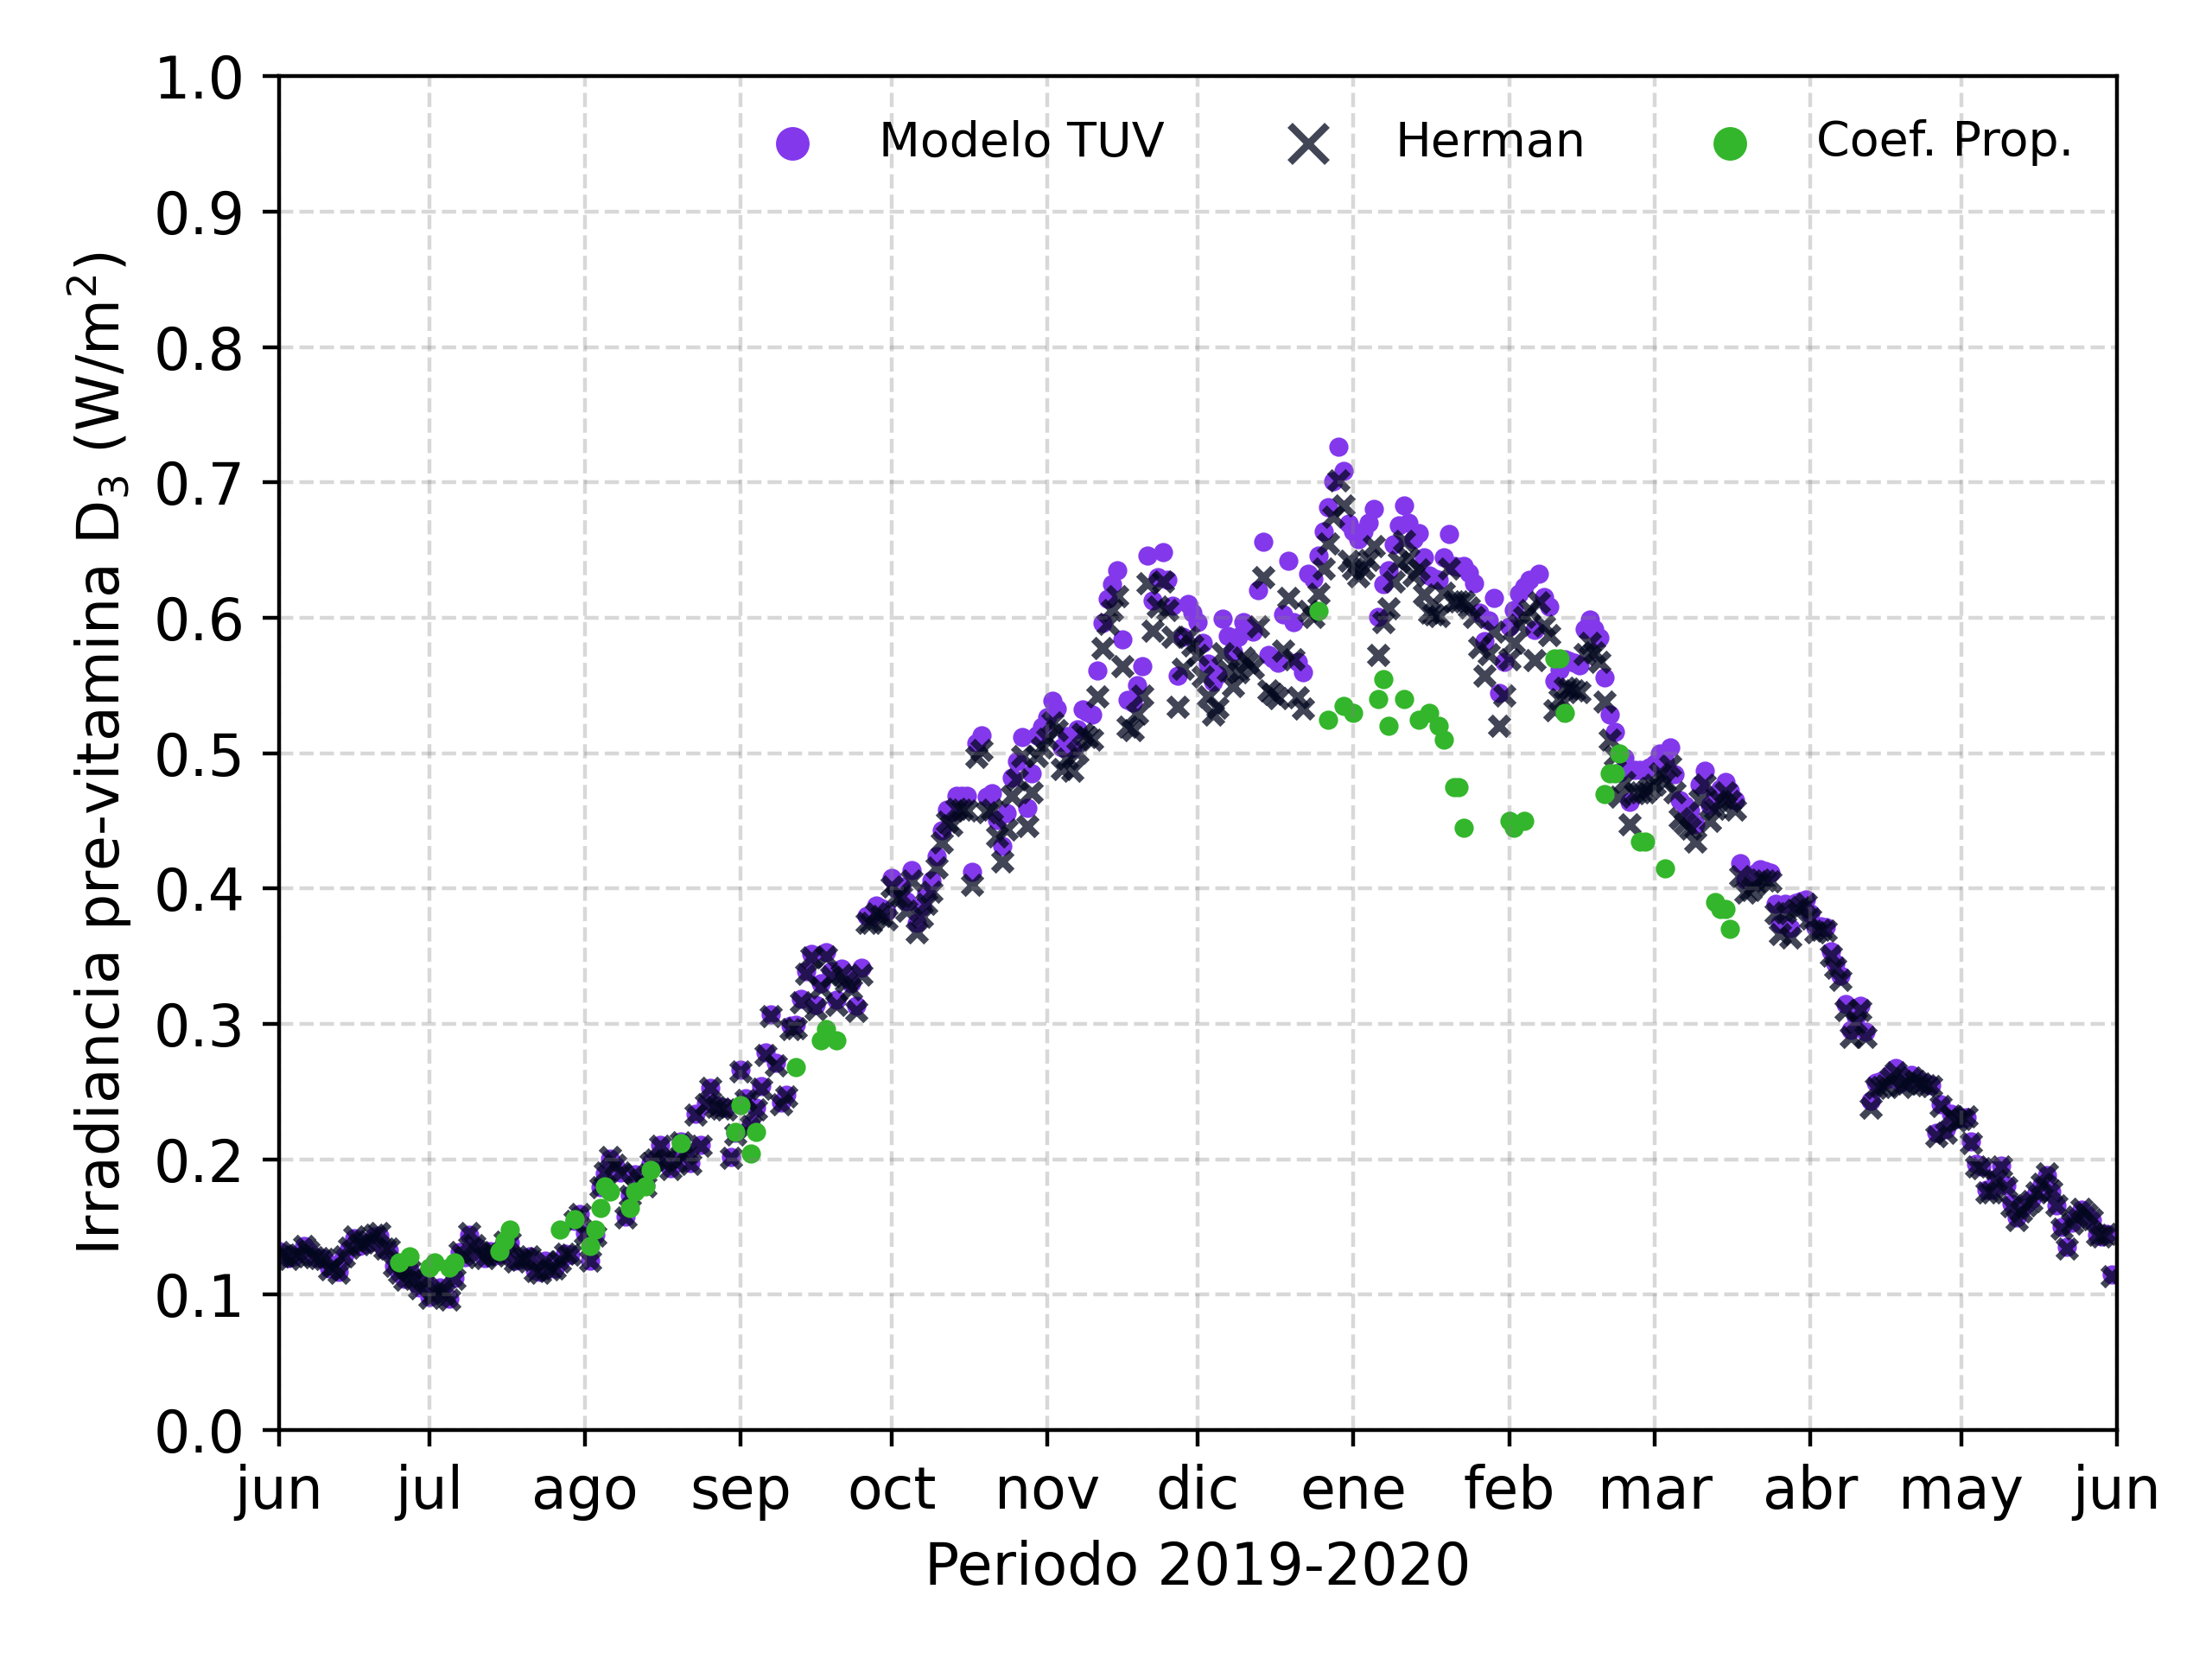
\includegraphics[scale=0.47]{Max_previtamin_D.png}
  \caption{E\textsubscript{vitD} para la ciudad de Rosario obtenida con el Coeficiente de proporcionalidad, Ec. de Herman y Modelo TUV.}
  \label{fig:previtamin}
\end{figure}
\begin{table*}[ht]
  \tiny
  \centering
  \caption{TES en minutos para cada dosis (x: no alcanzada) y fototipos obtenidos por Cabrera 2005 y Diaz et al. 2011 (celdas grises). Análisis del presente trabajo (celdas blancas) en un día de verano e invierno para acumular 1MED, $\frac{1}{4}$MED y 1MDD.}
  \begin{tabular}{|c|c|c|c|c|c|c|c|c|c|c|c|c|}
    \hline
                               & \multicolumn{4}{c|}{\begin{tabular}[c]{@{}c@{}}Diaz et al. 2011 \\ fototipo II\end{tabular}}         & \multicolumn{2}{c|}{\begin{tabular}[c]{@{}c@{}}Cabrera 2005\\ fototipo III\end{tabular}}                           & \multicolumn{6}{c|}{\begin{tabular}[c]{@{}c@{}}Presente\\ fototipo II\end{tabular}}                                                                                                                                                                                                                                                                                              \\ \cline{2-13}
                               & \multicolumn{2}{c|}{1MED (250 J/m\textsuperscript{2})} & \multicolumn{2}{c|}{1SDD\textsubscript{SA} (321 J/m\textsuperscript{2})} & \multicolumn{2}{c|}{1MED (210 J/m\textsuperscript{2})} & \multicolumn{2}{c|}{1MED (250 J/m\textsuperscript{2})} & \multicolumn{2}{c|}{$\frac{1}{4}$MED (63 J/m\textsuperscript{2})} & \multicolumn{2}{c|}{1MDD (136 J/m\textsuperscript{2})}                                                                                                 \\ \cline{2-13}
    \multirow{-3}{*}{Ciudad}   & verano                                                 & invierno                                                                 & verano                                                 & invierno                                               & verano                                                            & invierno                                               & verano & invierno                  & verano                    & invierno & verano & invierno \\ \hline
    \begin{tabular}[c]{@{}c@{}}Santiago\\ de Chile\end{tabular} & \cellcolor[HTML]{DAD7D7}21                             & \cellcolor[HTML]{DAD7D7}119                                              & \cellcolor[HTML]{DAD7D7}   12                          & \cellcolor[HTML]{DAD7D7}73                             & \cellcolor[HTML]{DAD7D7}10                                        & \cellcolor[HTML]{DAD7D7}56                             & 16     & 52                        & 4                         & 14       & 4      & 14       \\ \hline
    Rosario                    & -                                                      & -                                                                        & -                                                      &                                                        & -                                                                 & -                                                      & 14     & 52                        & 2                         & 12       & 2      & 16       \\ \hline
    \begin{tabular}[c]{@{}c@{}}Punta\\ Arenas\end{tabular} & \cellcolor[HTML]{DAD7D7}37                             & \cellcolor[HTML]{DAD7D7}x                                                & \cellcolor[HTML]{DAD7D7}24                             & \cellcolor[HTML]{DAD7D7}x                              & \cellcolor[HTML]{DAD7D7}26                                        & \cellcolor[HTML]{DAD7D7}134                            & 22     & \cellcolor[HTML]{FFFFFF}x & \cellcolor[HTML]{FFFFFF}4 & 92       & 8      & 192      \\ \hline
  \end{tabular}
  \label{table:TES}
\end{table*}
Un estudio\cite{LuChenHolick_2019} sobre el porcentaje de conversión de 7-DHC a pre-vitamina D\textsubscript{3} en diferentes latitudes y épocas del año, reveló que a latitudes mayores de $40^\circ$[S-N] en invierno, esta conversión es extremadamente ineficiente. La magnitud de este porcentaje es inversamente proporcional a la latitud en ciudades del continente americano. El máximo porcentaje de conversión a pre-vitamina D\textsubscript{3} en Buenos Aires y Ushuaia lo alcanzaron en diciembre. Este antecedente es semejante a los resultados obtenidos con los tres métodos de derivación de la E\textsubscript{vitD} en Rosario, ya que el máximo valor ocurre en diciembre (Fig. \ref{fig:previtamin}).

Para una exposición a partir del mediodía solar, en el periodo junio 2019 - mayo 2020 se estimaron los TES hasta alcanzar las diferentes dosis (Fig. \ref{fig:TES}). En invierno los TES para alcanzar 1 MDD, se encuentran en promedio a los 14$\pm$5 minutos, mientras que para acumular $\frac{1}{4}$MED a los 11$\pm$3 minutos y para la aparición de eritema (1 MED) a los 47$\pm$15 minutos. En verano, en promedio se requieren 4$\pm$1 min para alcanzar la dosis mínima de pre-vitamina D\textsubscript{3}, para $\frac{1}{4}$MED 4$\pm$1 min y 15$\pm$2 min para la eritémica. Los TES para obtener 1 MDD y $\frac{1}{4}$MED tuvieron valores semejantes, con una diferencia promedio de 1 min en ambas temporadas.

Para extender el análisis a otras latitudes, se incorporaron los valores de los TES obtenidos por dos estudios\cite{Diaz2011,cabrera_radiacion_2005}. Estos TES se muestran en la Tabla \ref{table:TES} para los fototipos y dosis. Diaz et al. 2011 considera una SDD\textsubscript{SA} (ponderada por el espectro de vitamina D\textsubscript{3}), para una exposición del 9\% del cuerpo (sólo la cabeza). Los valores para las ciudades de Santiago de Chile y Punta Arenas, también fueron estimados con el modelo TUV en dos fechas particulares de verano e invierno. Los TES para acumular un MED, en los tres estudios mostraron una ligera concordancia. Sin embargo, en invierno Punta Arenas no alcanzó la dosis, excepto en lo obtenido por Cabrera, posiblemente porque la dosis considerada es menor a las otras. Los TES en Santiago de Chile para acumular un MDD, fueron más largos en el trabajo de Díaz et al. 2011 que en el presente estudio. El mismo trabajo reveló que 1 MDD para Buenos Aires en verano, es alcanzada a los 13 min. A pesar de que esta ciudad se encuentra a 300 km de Rosario, los TES se extienden también poco más del triple respecto al promedio obtenido con el modelo TUV (4$\pm$1 min). Esta diferencia se debe a que en nuestras estimaciones se considera un área de piel expuesta mayor (25\% del cuerpo).

\begin{figure}[ht]
  \centering
  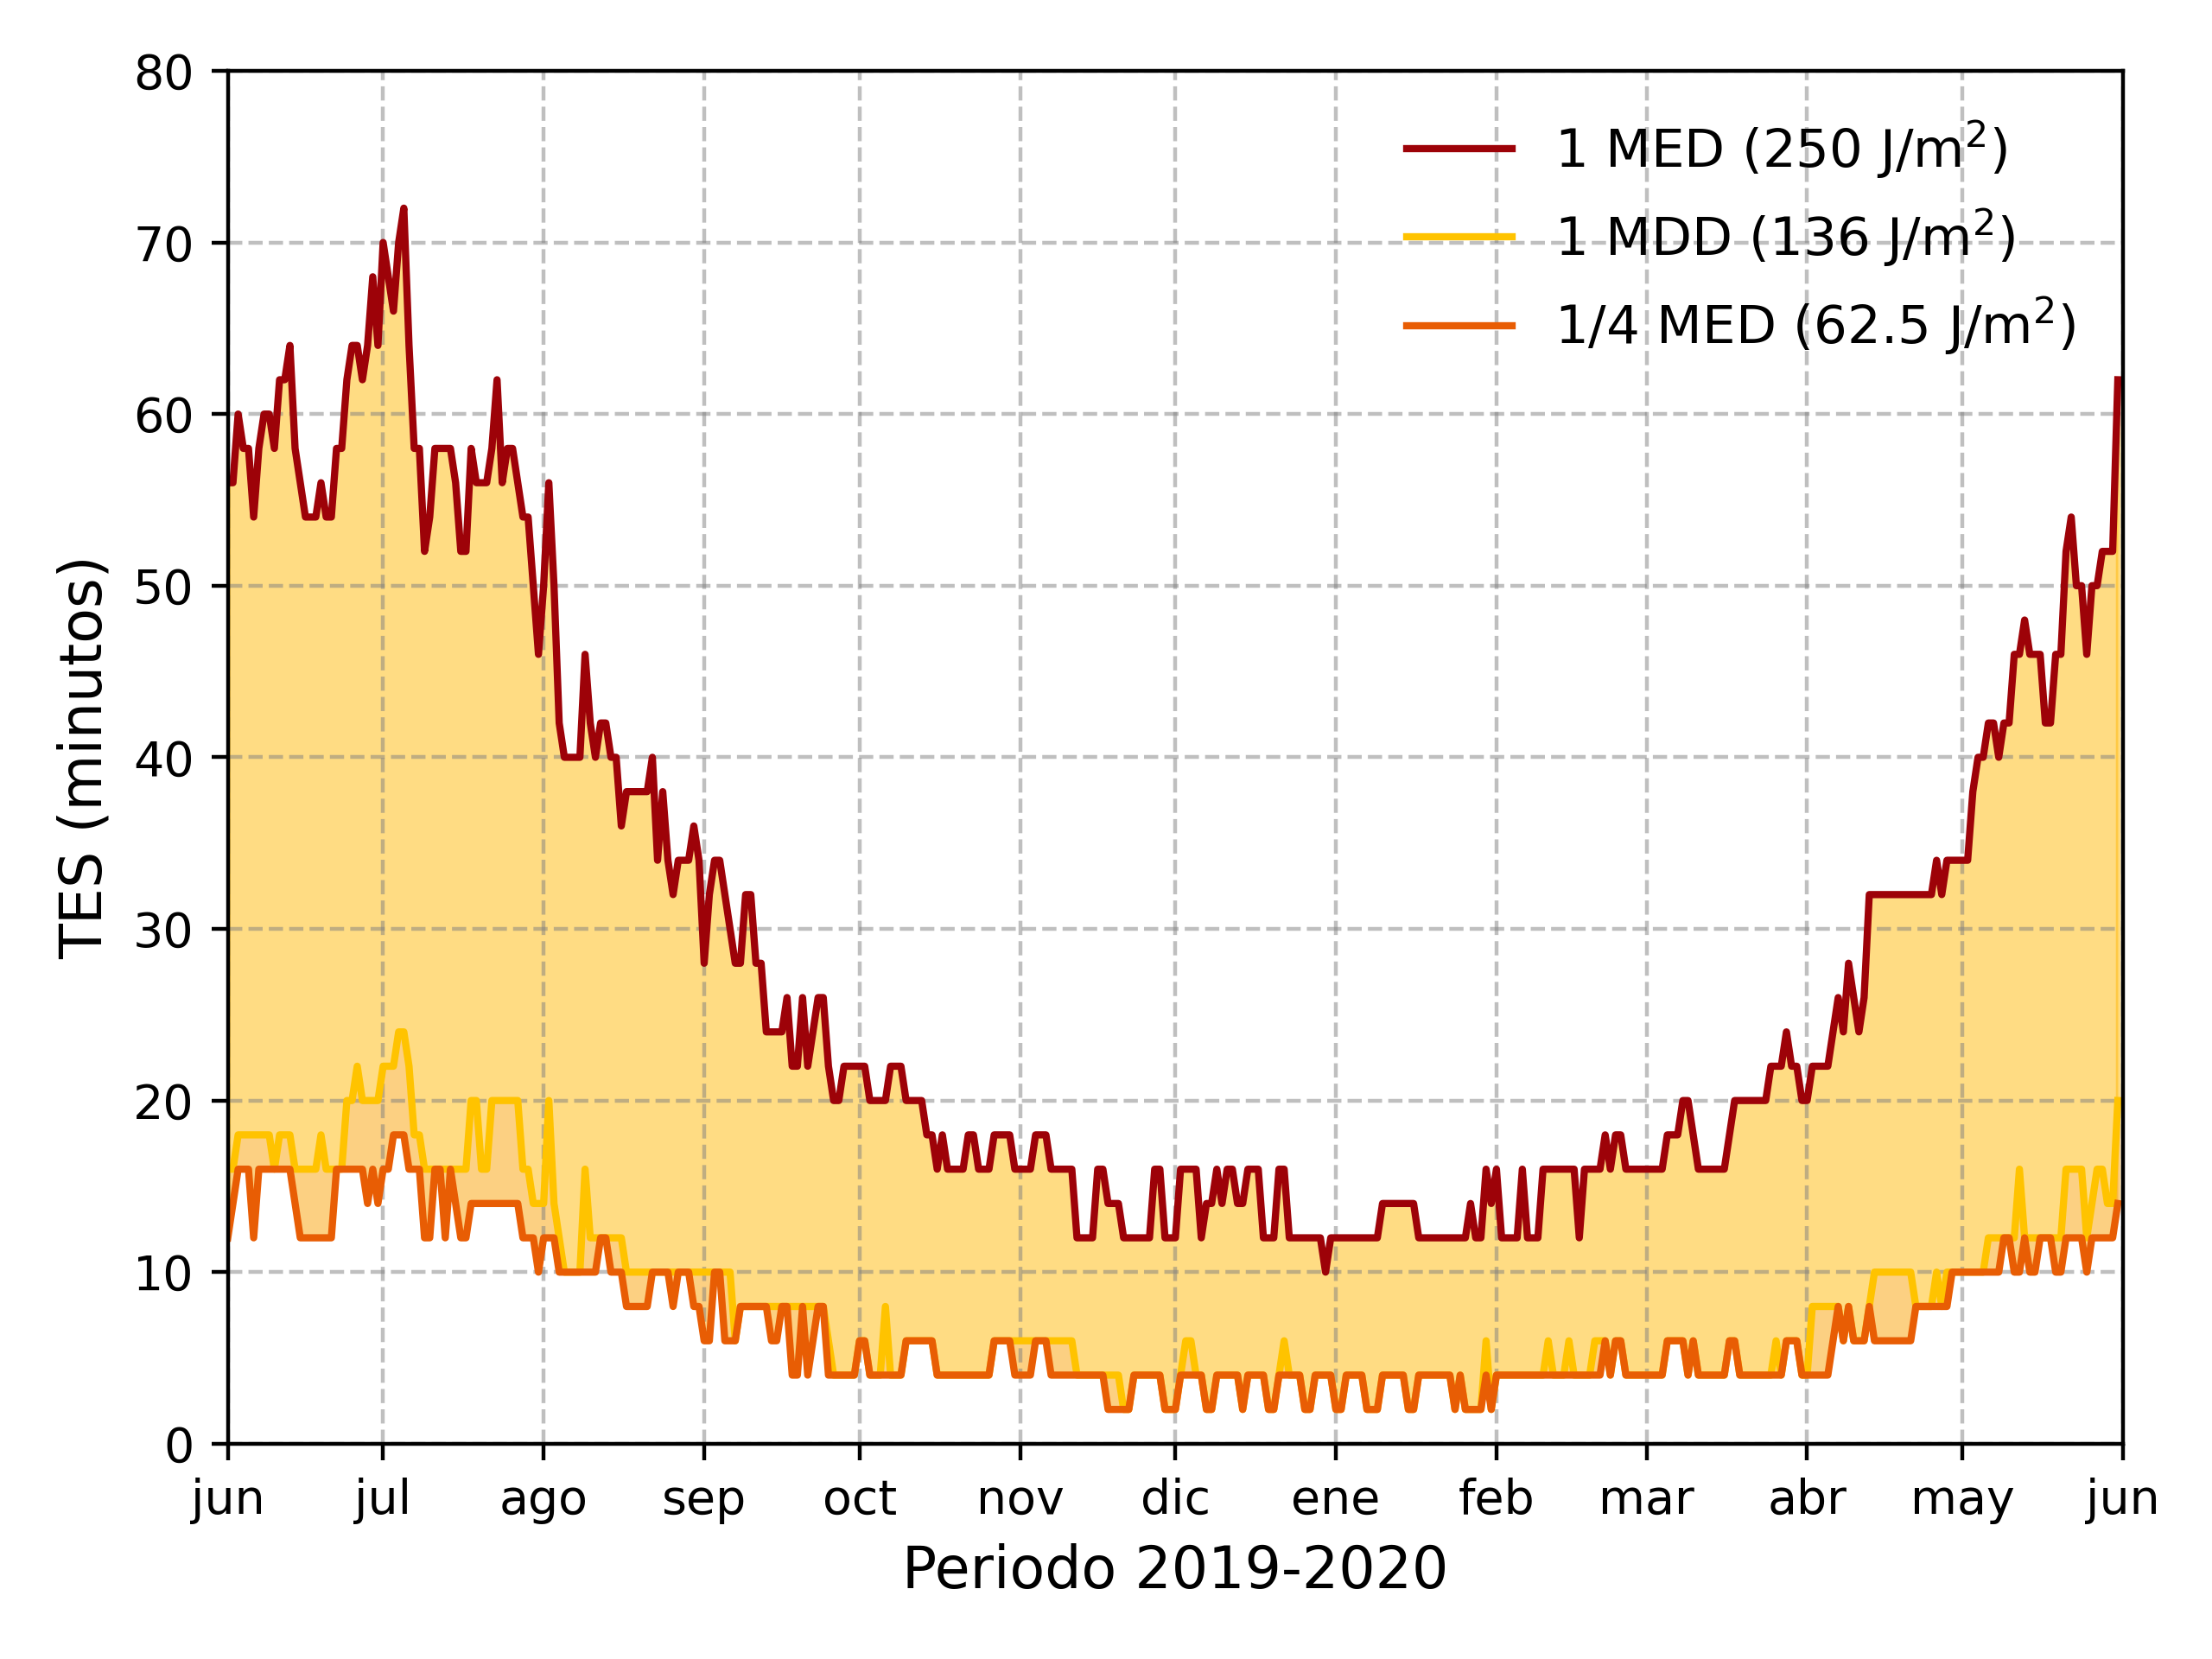
\includegraphics[scale=0.47]{dosis_vitamin.png}
  \caption{TES diarios para acumular $\frac{1}{4}$MED, 1MDD y 1MED en una persona de un fototipo de piel II comenzando la exposición a partir del mediodía solar.}
  \label{fig:TES}
\end{figure}

\section{DISCUSIÓN Y CONCLUSIONES}
El modelo TUV y la Ec. de Herman mostraron valores semejantes de E\textsubscript{vitD} debido a que ambos métodos consideran el O\textsubscript{3} y el $\theta$ como principales elementos de influencia. Sin embargo, los aerosoles atenúan la radiación solar UV y podrían afectarla de manera importante cuando tienen lugar incendios en el Delta del río Paraná frente a Rosario.\cite{IPINA2012966} Respecto a los valores derivados del Coeficiente de proporcionalidad, aunque su aplicación es práctica, la aproximación depende del factor $k$ de cada época del año.

El análisis comparativo de los TES para las MDD reveló que las principales diferencias se deben a los siguientes factores: 1) la superficie expuesta del cuerpo (relacionada al valor de la dosis), 2) las condiciones de cielo (despejado o nublado) y 3) la presencia de contaminación atmosférica. Por otro lado, estimamos que un MED en Rosario se alcanza en promedio a los 15$\pm$2 min en verano, los cuales se encuentran en el rango esperado de acuerdo a la latitud. Los TES calculados para una MDD y $\frac{1}{4}$MED indicaron una diferencia promedio entre ambos de 0.5 min en verano y 3 min en invierno. Por lo tanto, es posible derivar los TES con relativa precisión, a partir de la estimación de un MED.

El modelo TUV, la Ec. de Herman y el Coeficiente de proporcionalidad estiman valores de E\textsubscript{vitD} para cielo despejado, en consecuencia estos TES podrían ser considerados como un límite de tiempo mínimo de la exposición al sol, mientras que los TES para acumular un MED pueden ser tomados como límite de tiempo superior. De esta manera, podríamos obtener niveles adecuados de vitamina D, evitando las consecuencias en la Salud que provoca su deficiencia, sin los efectos nocivos que conlleva la sobreexposición solar. Este estudio podría extenderse en un futuro para analizar la contribución de los aerosoles troposféricos, así como la mezcla en altura con la capa límite atmosférica en eventos de quema de biomasa.
\section{REFERENCIAS}
%\bibliographystyle{abbrv} %orden alfabético 
\bibliographystyle{aichej} %orden de mención
\renewcommand{\refname}{}
\bibliography{references}
\end{document}